\documentclass[10pt]{article}
\usepackage[letterpaper,left=0.7in,right=0.7in,top=0.5in,bottom=0.5in]{geometry}
\usepackage[T1]{fontenc}
\usepackage{lmodern}
\usepackage{amsmath,amssymb}
\usepackage{microtype}
\usepackage{booktabs,array,tabularx}
\usepackage{xcolor}
\usepackage{tikz}
\usetikzlibrary{arrows.meta,positioning,fit,calc}
\setlength{\parindent}{0pt}
\setlength{\parskip}{2.5pt}
\pagestyle{empty}
\definecolor{accent}{HTML}{9B1B30}
\definecolor{soft}{HTML}{F3F3F3}
\newcommand{\head}[1]{\par\vspace{2pt}{\color{accent}\bfseries #1}\ }
\newcommand{\thm}[2]{\par\vspace{1pt}\colorbox{soft}{\parbox{\dimexpr\linewidth-2\fboxsep}{\textbf{#1.} #2}}\par}
\newcommand{\B}{\mathcal{B}}
\newcommand{\sat}{\operatorname{sat}}
\newcommand{\bkd}{\operatorname{backed}}
\newcommand{\fth}{\operatorname{faithful}}
\newcommand{\always}{\Box}
\newcommand{\lean}[1]{\texttt{#1}}
\newcolumntype{L}{>{\raggedright\arraybackslash}X}
\begin{document}
\fontsize{9.5pt}{11.4pt}\selectfont
\setlength{\abovedisplayskip}{3pt}\setlength{\belowdisplayskip}{3pt}\setlength{\abovedisplayshortskip}{2pt}\setlength{\belowdisplayshortskip}{2pt}

{\LARGE\bfseries The harness algebra}\hfill{\small 2026-11-18\quad Lean: \lean{Harness/Algebra.lean}, core Lean 4.35, 34 theorems, no \lean{sorry}}

\vspace{2pt}
A harness packages one module of real C++ as a triple: implementation, contract, evidence. Every definition and theorem on this page is in the Lean file. Page 2 applies the algebra to the tube theorem and is a plan, not a result.

\head{1. Contracts (recalled).} Fix a set $\B$ of behaviors: runs of every signal of the system, tick by tick. Implementations, assumptions and guarantees are subsets of $\B$, and a contract is a pair $C=(A,G)$.
\begin{gather*}
M\models C \iff M\cap A\subseteq G,\qquad \sat C = G\cup A^{c},\qquad C_1\preceq C_2 \iff A_2\subseteq A_1 \ \text{and}\ \sat C_1\subseteq \sat C_2,\\
C_1\otimes C_2=\bigl((A_1\cap A_2)\cup(\sat C_1\cap \sat C_2)^{c},\ \sat C_1\cap \sat C_2\bigr),\qquad
C_1\wedge C_2=\bigl(A_1\cup A_2,\ \sat C_1\cap \sat C_2\bigr),\\
C/C_1=\bigl(A\cap \sat C_1,\ \sat C\cap A_1\bigr),\qquad \pi^{*}C'=(\pi^{-1}A',\ \pi^{-1}G')\ \ \text{for a projection } \pi:\B\to\B' \text{ onto an interface.}
\end{gather*}
Facts used below: $M_1\models C_1$ and $M_2\models C_2$ give $M_1\cap M_2\models C_1\otimes C_2$; refinement preserves implementation; $\otimes$ is monotone, commutative and associative; $\wedge$ is the greatest lower bound; $C_1\otimes X\preceq C \iff X\preceq C/C_1$; and $M\models\pi^{*}C' \iff \pi(M)\models C'$.

\head{2. Harness.} A harness is $H=(M,C,E)$. $M\subseteq\B$ is the set of runs the module's executable can produce; Lean never defines it, it is a variable. $C$ is a contract. $E$ is evidence for the claim $M\models C$, a tree:
\[
E \ ::=\ \mathsf{leaf}(r)\ \mid\ \mathsf{derive}(E,\,h)\ \mid\ E\wedge E\ \mid\ \textstyle\bigwedge_{i<n}E_i\ \mid\ E\vee E .
\]
A leaf is a ledger record $r$ offered for a claim: its kind (proved by a model checker, tested, monitored, assumed) and the hashes of the code, the clause and the result. Lean cannot check it. $\mathsf{derive}(E,h)$ holds a Lean proof $h$ that the claim follows from the one $E$ supports. $\wedge$ collects evidence for several claims; $\vee$ is a second, independent support for the same claim.

A \emph{policy} $T$ is the set of records a reader accepts, for example ``proved, with current hashes'' or ``proved or tested''. Evidence is read under a policy in two ways. $\bkd_T(E)$: the tree reaches its claim through accepted records only ($\mathsf{leaf}(r)$: $r\in T$; $\wedge$: all children; $\vee$: some child; $\mathsf{derive}$: the child). $\fth_T(E)$: every accepted record in the tree is true of its claim.

\thm{Theorem 1 (soundness)}{If $\fth_T(E)$ and $\bkd_T(E)$, then $M\models C$. With $T=\emptyset$, $\bkd_T(E)$ alone gives $M\models C$: the claim is a Lean theorem. \ \lean{Ev.sound}, \lean{Harness.sound}, \lean{Ev.proved\_of\_supported\_empty}}

$\fth_T$ is exactly what a system claim takes on trust. A stale record (code or clause changed) is one the policy no longer accepts.

\head{3. Operations.} Each returns a harness. The proof inside each $\mathsf{derive}$ node is a theorem of the contract algebra.

{\footnotesize\renewcommand{\arraystretch}{1.05}
\begin{tabularx}{\linewidth}{@{}l l l l L@{}}
\toprule
Operation & Implementation & Contract & Evidence & Side condition, proved in Lean\\
\midrule
leaf & $M$ & $C$ & $\mathsf{leaf}(r)$ & none\\
compose $H_1\otimes H_2$ & $M_1\cap M_2$ & $C_1\otimes C_2$ & $\mathsf{derive}(E_1\wedge E_2)$ & none\\
refine $H$ to $C'$ & $M$ & $C'$ & $\mathsf{derive}(E)$ & $C\preceq C'$\\
conjoin & $M$ & $C\wedge C_2$ & $\mathsf{derive}(E\wedge E_2)$ & none; $E_2$ is evidence for $M\models C_2$\\
second support & $M$ & $C$ & $E\vee E'$ & none; $E'$ is evidence for the same claim\\
hide through $\pi$ & $\pi(M)$ & $C'$ & $\mathsf{derive}(E)$ & $C\preceq\pi^{*}C'$\\
fill (quotient) & $M_1\cap M_2$ & $C$ & $\mathsf{derive}(E_1\wedge E_2)$ & $C_2\preceq C/C_1$\\
loop (section 5) & $\bigcap_i M_i$ & $\always(e,\bigwedge_i g_i)$ & $\mathsf{derive}(\bigwedge_i E_i)$ & $C_i\preceq\always(a_i,g_i)$ and the discharge condition of Theorem 2\\
\bottomrule
\end{tabularx}}

\head{4. Laws.}
\textbf{(L1) Projection.} $H\mapsto C$ commutes with every operation, and $H\mapsto M$ sends $\otimes$ to $\cap$, so every law of section 1 holds for harnesses.
\textbf{(L2) Weakest link.} $\bkd_T(H_1\otimes H_2)\iff\bkd_T(H_1)$ and $\bkd_T(H_2)$; a loop is backed exactly when all its modules are; refine and hide leave $\bkd_T$ unchanged; a second support gives $\bkd_T(E)$ or $\bkd_T(E')$; and $\bkd_T$ grows with $T$.
\textbf{(L3) Swap.} Replacing $H_1$ by $H_1'$ with the same contract leaves every ancestor's contract unchanged; with a refining contract, the composite's contract is refined. No proof above the leaf mentions $M$, so only the leaf record is new.
\textbf{(L4) Closure.} A composite is a harness: it can be a child of a larger one, or be tested as a unit (a second support).

\head{5. Ticks: step contracts and the loop rule.} Module contracts are stated per tick. A step contract is $S=(a,g)$ with $a,g\subseteq\B\times\mathbb{N}$. Its reading over runs puts everything in the guarantee: $\always S=\bigl(\B,\ \{\,b : \forall t,\ (\forall s\le t,\ a(b,s))\Rightarrow g(b,t)\,\}\bigr)$. A per-tick monitor, or a test campaign on one module alone, checks the stronger $a(b,t)\Rightarrow g(b,t)$.

\thm{Theorem 2 (loop rule)}{Let modules $M_0,\dots,M_{n-1}$ run in this order within a tick, with $M_i\models\always(a_i,g_i)$, and let $e\subseteq\B\times\mathbb{N}$ be the environment's assumption. Suppose that for every run $b$, tick $t$ and module $i$: if $e$ holds up to $t$, $g_j(b,t)$ holds for every $j<i$, and $g_j(b,s)$ holds for every $j$ and every $s<t$, then $a_i(b,t)$. Then $\bigcap_i M_i\models\always(e,\ \bigwedge_i g_i)$. \ \lean{loop}, \lean{loop\_two}, \lean{Harness.loop}}

The condition never uses a same-tick guarantee of a module scheduled later: that is ``no instantaneous loop''. Feedback is discharged through earlier ticks (the plant's assumption at $t$ is about the commands at $t-1$). The result is again a step contract, so loops nest. Without ticks the rule fails: around a loop, $(\always a_1,\always g_1)$ and $(\always a_2,\always g_2)$ leave each assumption resting on the other's guarantee.

\head{6. Compared with the contract algebra.} On contracts the two coincide (L1). The harness algebra adds: (i) \emph{evidence}, where the contract algebra has only $M\models C$ true or false, and a computation of which records a system claim rests on; (ii) \emph{opaque implementations}: $M$ is an executable, so a leaf claim is a record, never a Lean proof, and every proof above the leaves mentions no code; (iii) \emph{ticks}: step contracts and the loop rule, which make feedback sound.

\head{Status.} Formalized: all of the above. Built in the runner: one module (\lean{rate\_pid}), isolated test campaigns, the hash-bound ledger. Not built: any composite, and the link from the runner's binary32 clause language to the sets $a$, $g$.

\newpage
{\LARGE\bfseries Decomposing the tube theorem}\hfill{\small a plan; nothing here is proved or built unless marked}

\vspace{2pt}
\head{Target.} With sensor noise bounded by $\nu$, the vehicle stays within $\rho(\nu)$ of the reference: $C_{\mathrm{sys}}=\always(e,g)$ with $e(t)$: $\|y(t)-h(x(t))\|\le\nu$, the plan is well formed, the start is at rest on the path, no failsafe input fires; and $g(t)$: $\|p(t)-p_r(t)\|\le\rho$. Guidance guarantees that $p_r(t)$ lies on the planned path, so the distance from the vehicle to the path is at most $\rho$.

\begin{center}
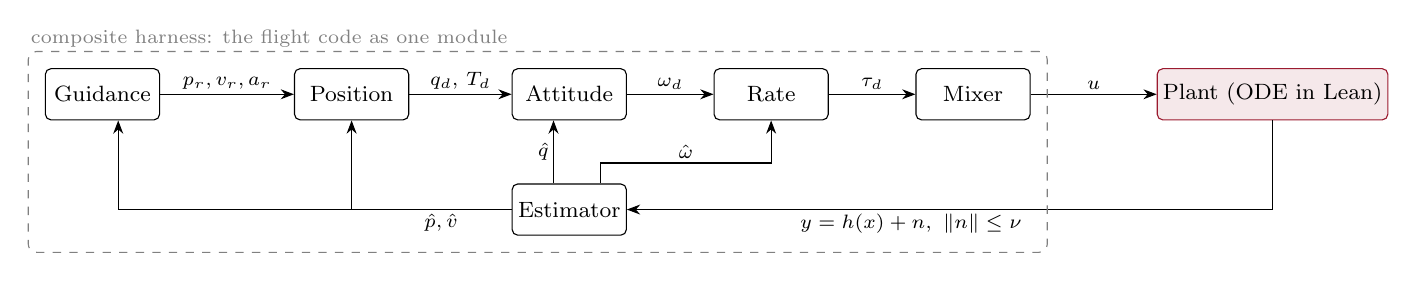
\begin{tikzpicture}[font=\footnotesize,>=Stealth,
  m/.style={draw,rounded corners=2pt,minimum height=6.5mm,minimum width=14.5mm,fill=white,inner sep=2pt},
  pl/.style={m,fill=accent!10,draw=accent},
  lab/.style={font=\scriptsize,inner sep=1.5pt}]
\node[m] (gd) {Guidance};
\node[m,right=17mm of gd] (pos) {Position};
\node[m,right=13mm of pos] (att) {Attitude};
\node[m,right=11mm of att] (rate) {Rate};
\node[m,right=11mm of rate] (mix) {Mixer};
\node[pl,right=16mm of mix] (plant) {Plant (ODE in Lean)};
\node[m,below=8mm of att] (est) {Estimator};
\draw[->] (gd)--node[lab,above]{$p_r,v_r,a_r$}(pos);
\draw[->] (pos)--node[lab,above]{$q_d,\,T_d$}(att);
\draw[->] (att)--node[lab,above]{$\omega_d$}(rate);
\draw[->] (rate)--node[lab,above]{$\tau_d$}(mix);
\draw[->] (mix)--node[lab,above]{$u$}(plant);
\draw[->] (plant.south)|-node[lab,pos=0.78,below]{$y=h(x)+n,\ \|n\|\le\nu$}(est.east);
\draw[->] (est.west)-|node[lab,pos=0.22,below]{$\hat p,\hat v$}(pos.south);
\draw[->] (est.west)-|($(gd.south)+(2mm,0)$);
\draw[->] ($(est.north)+(-2mm,0)$)--node[lab,left]{$\hat q$}($(att.south)+(-2mm,0)$);
\draw[->] ($(est.north)+(4mm,0)$)--++(0,2.6mm)-|node[lab,pos=0.25,above]{$\hat\omega$}(rate.south);
\node[draw,dashed,gray,rounded corners=3pt,fit=(gd)(mix)(est),inner sep=6pt,label={[gray,font=\scriptsize,anchor=south west,inner sep=1pt]north west:composite harness: the flight code as one module}] {};
\end{tikzpicture}
\end{center}

\vspace{-4pt}
\head{Two kinds of clause.} A \emph{range} clause keeps a module's outputs in a set while its inputs are in one (lean angle at most $\bar\theta$, $\|\omega_d\|\le\Omega$, $u\in[0,1]^4$); it discharges the neighbors' assumptions. A \emph{conformance} clause puts the output within $\delta_i$ of a reference law $\kappa_i$ over the reals, on the same inputs and exposed state: $\|\mathrm{out}-\kappa_i(\mathrm{in},\mathrm{state})\|\le\delta_i$. It is what stands in for the code: Lean reasons about $\kappa_i$ plus a disturbance of size $\delta_i$. Both are one-run, per-tick clauses, so each can be tested on the module alone and monitored in flight.

\head{Contracts per module.} Each is a step contract; $\mathcal{E}$ is a flight envelope (bounds on speed, acceleration, tilt and body rates).

{\footnotesize\renewcommand{\arraystretch}{1.05}
\begin{tabularx}{\linewidth}{@{}>{\raggedright\arraybackslash}p{3.95cm} >{\raggedright\arraybackslash}p{3.3cm} >{\raggedright\arraybackslash}p{5.5cm} L@{}}
\toprule
Module (C++) & Assumes & Guarantees & Excited alone by\\
\midrule
Estimator (\lean{AP\_NavEKF3}) & noise $\le\nu$; true motion in $\mathcal{E}$ & $\|\hat p-p\|\le\varepsilon_p$, $\|\hat v-v\|\le\varepsilon_v$, $\angle(\hat q,q)\le\varepsilon_q$, $\|\hat\omega-\omega\|\le\varepsilon_\omega$ & truth runs in $\mathcal{E}$, synthesized samples; truth is a ghost input\\
Guidance (\lean{AC\_WPNav}) & plan well formed & $p_r$ on the path; $\|v_r\|\le V$, $\|a_r\|\le A$ & generated plans and estimates\\
Position (\lean{AC\_PosControl}) & reference bounds; errors in range & $a_d$ within $\delta_{\mathrm{pos}}$ of $\kappa_{\mathrm{pos}}$; tilt of $q_d\le\bar\theta$; $T_d$ in range & inputs inside the assumption\\
Attitude (\lean{AC\_AttitudeControl}) & tilt $\le\bar\theta$; error in range & $\omega_d$ within $\delta_{\mathrm{att}}$ of $\kappa_{\mathrm{att}}$; $\|\omega_d\|\le\Omega$ & same\\
Rate (three \lean{AC\_PID}) & $\|\omega_d\|,\|\hat\omega\|\le\Omega$; gains in range & $\tau_d$ within $\delta_{\mathrm{rate}}$ of $\kappa_{\mathrm{rate}}$; integrators bounded; no internal error & same; \textbf{built} for one PID: range clauses\\
Mixer (\lean{AP\_MotorsMatrix}) & $\tau_d$, $T_d$ unsaturated & $u\in[0,1]^4$; wrench of $u$ within $\delta_{\mathrm{mix}}$ of $(\tau_d,T_d)$ & same\\
Supervisor (modes, failsafes) & health inputs nominal & mode stays Auto; the schedule runs every tick & event sequences; monitored\\
Plant (ODE in Lean) & $u\in[0,1]^4$; state in $\mathcal{E}$ & $x(t)$ is the exact flow from $x(t-1)$ under $u(t-1)$ & Lean theorem; simulator gap measured\\
\bottomrule
\end{tabularx}}

\head{Composition, in Lean, with no code.}
\textbf{Step 1, the loop.} ArduCopter's own order within a tick is rate, mixer, estimator, guidance, position, attitude, with the plant between ticks; the rate controller uses the attitude controller's target of the previous tick. Theorem 2 applies with that order. Its discharge condition is a finite list of inequalities between the constants above (the budget closes: for example $\bar\theta$ plus the attitude error stays inside $\mathcal{E}$). It yields that every clause in the table holds at every tick while $e$ holds.

\textbf{Step 2, three gain lemmas over the reals}, about the $\kappa_i$ and the ODE, one per nested loop, each $\Gamma$ monotone:
\[
\underbrace{\|\omega-\omega_d\|\le\Gamma_\omega(\varepsilon_\omega,\delta_{\mathrm{rate}},\delta_{\mathrm{mix}})}_{\text{rate loop}=:\ \varepsilon_{\mathrm{rate}}}\qquad
\underbrace{\angle(q,q_d)\le\Gamma_q(\varepsilon_q,\varepsilon_{\mathrm{rate}},\delta_{\mathrm{att}})}_{\text{attitude loop}=:\ \varepsilon_{\mathrm{att}}}\qquad
\underbrace{\|p-p_r\|\le\Gamma_p(\varepsilon_p,\varepsilon_v,\varepsilon_{\mathrm{att}},\delta_{\mathrm{pos}},A)}_{\text{position loop}}
\]
\[
\rho(\nu)=\Gamma_p\bigl(\varepsilon_p(\nu),\ \varepsilon_v(\nu),\ \Gamma_q(\varepsilon_q(\nu),\ \Gamma_\omega(\varepsilon_\omega(\nu),\delta_{\mathrm{rate}},\delta_{\mathrm{mix}}),\ \delta_{\mathrm{att}}),\ \delta_{\mathrm{pos}},\ A\bigr).
\]
\textbf{Step 3.} Refine the loop's contract to $C_{\mathrm{sys}}$ and hide the internal signals. Read the other way, the quotient of $C_{\mathrm{sys}}$ by the parts already backed is the specification of the remaining part, for example the error budget $(\varepsilon_p,\varepsilon_v,\varepsilon_q,\varepsilon_\omega)$ the estimator is allowed.

\head{Evidence.} \textbf{Leaves.} One isolated campaign per clause. It records the largest error seen ($\hat\varepsilon_i$, $\hat\delta_i$) and the smallest margin; the constant in the contract is set above it. The rate controller and the mixer are small enough to try a model checker, which would make their records \emph{proved}. \textbf{Top level.} The composite is a module (L4), so it gets its own harness: closed loop with the simulator, excited by noise sequences bounded by $\nu$, random and adversarial. It monitors every inner clause each tick, which checks in flight that each assumption is discharged, and the system clause, giving an observed $\hat\rho\le\rho$; $\rho/\hat\rho$ measures how conservative the theorem is. This is a second support for $C_{\mathrm{sys}}$. A top-level violation with no leaf violation would point at the plant model or the schedule.

\head{What is hard.}
(1) The gain lemmas are the control theory (a nonlinear cascade with saturation). None is proved for the X500; the plant library has the per-period sensitivity they need, not the multi-period one.
(2) The estimator carries all the dependence on $\nu$, and its contract will rest on tests and monitoring.
(3) Each $\kappa_i$ is a small real-valued model of a module, written in Lean; if it omits a filter or a limiter, $\delta_i$ is large.
(4) Guidance reads the position estimate, so $p_r$ moves with the noise; the tube is therefore around $p_r$ and the path. A tube around the noise-free run would need two-run (sensitivity) contracts, which the harness cannot yet check.
(5) Of the seven C++ modules, part of one exists: a single rate PID.
\end{document}
